\section{Computing initial values for pools of instances}

In \sbmlLthreeVone, \class{InitialAssignment}s are used to assign initial values to variables of a model, that are \class{Compartment}s, \class{Species}, \class{SpeciesReference}, or global \class{Parameter}s.  In order to assign the value of a specific type of species, \class{InitialAssignment}s in \multiVone also contain an element \class{SpeciesTypeInstanceChange}. The assignment sets the initial quantity of instances that fulfil a certain selection using the mathematical expression provided. The value provided by the \class{InitialAssignment} overides the value provided by the attributes \attribute{initialAmount} or \attribute{initialConcentration} of the relevant \class{SpeciesTypeInstance}.

\begin{figure}[h!]
\begin{center}
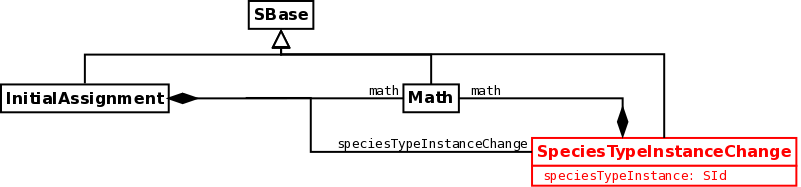
\includegraphics[scale=0.3]{./figs/pngs/InitialAssignmentGeneral.png}
\caption{\class{InitialAssignment} and all the associated classes of \multiVone.}
\end{center}
\end{figure}


\subsection{InitialAssignment}

In order to assign the initial values to entity subpools, defined by specific state and connectivity, the element \class{InitialAssignment} of \sbmlLthreeVone core is linked to a \class{SpeciesTypeInstanceChange}.

\begin{figure}[H]
\begin{center}
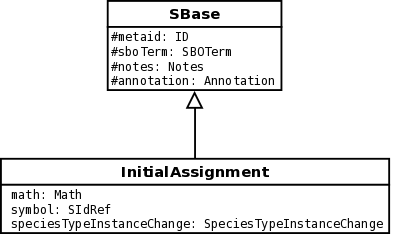
\includegraphics[scale=0.4]{figs/pngs/InitialAssignmentClass.png} 
\caption{Definition of the extended version of \class{InitialAssignment} and its relation with \class{SBase}.}
\label{fig:InitialAssignmentClass}
\end{center}
\end{figure}

\subsection{SpeciesTypeInstanceChange}\label{SpeciesTypeInstanceChange}

As all elements derived from \class{SBase}, A \class{SpeciesTypeInstanceChange} can link to \class{Notes} and \class{Annotation}, and carry a \attribute{metaid}, and an \attribute{sboTerm}. It targets a \class{SpeciesTypeInstance} through its \attribute{SpeciesTypeInstance} attribute. The change is computed using a MathML construct, as is always the case in \sbmlLthreeVone.

\begin{figure}[H]
\begin{center}
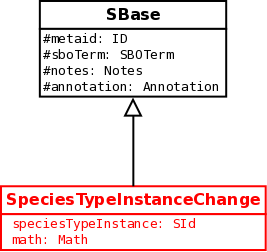
\includegraphics[scale=0.3]{figs/pngs/SpeciesTypeInstanceChangeClass.png} 
\caption{Definition of \class{SpeciesTypeInstanceChange} and its relation with \class{SBase}.}
\label{fig:SpeciesTypeInstanceChangeClass}
\end{center}
\end{figure}

\subsection{Complete example of an initial assignment}

The following example presents the assignment of the initial value for the subpool of \cdata{species1} defined as \cdata{speciesTypeInstance1}. This value is computed as the product of the parameters \cdata{x} and \cdata{y}, defined elsewhere. Note the empty \class{Math}, used when the software is unable to use the package \multiVone.

\begin{example}
<species id="species1" 
         boundaryCondition="false" hasOnlySubstanceUnit="false" constant="false"
         compartment="compartment1" initialAmount="1000"
         xmlns:multi="http://www.sbml.org/sbml/level3/version1/multi/version1"
         multi:speciesType="speciesType1" >
  <multi:listOfSpeciesTypeInstances>
    <multi:speciesTypeInstance multi:id="speciesTypeInstance1" multi:initialAmount="1">
      <multi:listOfSelectorReferences>
        <multi:selectorReference multi:selector="selector1" />
      <multi:listOfSelectorReferences>
    </multi:speciesTypeInstance>
  </multi:listOfSpeciesTypeInstances>
</species>
<initialAssignment symbol="species1">
  <multi:speciesTypeInstanceChange speciesTypeInstance="speciesTypeInstance1">
    <math xmlns="http://www.w3.org/1998/Math/MathML">
      <apply>
        <times/>
        <ci> x </ci>
        <ci> y </ci>
      </apply>
    </math>
  </multi:speciesTypeInstanceChange>
  <math xmlns="http://www.w3.org/1998/Math/MathML" />
</initialAssignment>
\end{example}